\chapter{POLARIZABILITY MEASUREMENTS OF NA, K, AND RB}
\label{polChapter}

As introduced in Chapter 2, we measured the absolute and relative polarizabilities of sodium, potassium, and rubidium using a Mach-Zehnder atom interferometer with an electric-field gradient. Table \ref{polResultsTable} shows the absolute measurements (which have less than 1.0\% uncertainty), and Table \ref{polRatiosTable} shows the ratios of polarizability measurements (which we measured with 0.3\% precision). 


Our paper published in \emph{Physical Review A}, and shown in Appendix \ref{polPRAappendix}, explains the most important details of the experiment. In this chapter I provide supporting material. I explain how I improved the accuracy of the velocity measurements, I provide a reanalysis of the data set after discarding outliers, and I discuss subsequent improvements that I made to the polarizability measurement interaction region and data acquisition system.






%%%%%%%%%%%%%%%%%%%%%%%%%%%%%%%%%%%%
\section{Improved velocity measurement using a length gauge to study diffraction}
\label{polLG}
Section \ref{polBrief} described how the atom beam velocity was measured by studying diffraction data (see Figure \ref{nakrbDiffraction}). This technique determines the de Broglie wavelength of atoms in the beam, but it relies on accurate knowledge of the displacement of the hot-wire detector. The DC motors used to move components in our atom beam machine, including the detector translation stage, report their position using rotary encoders and knowledge of the screw pitch as a proxy for linear displacement. However, because of variations in the screw pitch and stick/slip behavior in the translation stage, these position reports are subject to as much as 15 $\mu$m errors in linear displacement of the translation stage. Since the diffraction orders are typically spaced by about 130 $\mu$m, this corresponds to a $\sim$10\% error in velocity. Figure \ref{intRegionMotorLG} shows the displacement reported by a typical motor vs the displacement reported by a length gauge.


To overcome this problem, I installed a Heidenhain MT-2571 length gauge to measure the detector displacement using a linear encoder. Figure \ref{velMotLG} shows atom beam velocities and velocity distribution widths determined by fitting diffraction data when using either the length gauge or the motor encoder to measure the detector position. The velocity measurement is clearly more reproducible when using the length gauge to measure detector displacement. I also note that it is possible that detector position measurement errors were significant and neglected in the Ekstrom \etal measurement of sodium polarizability \cite{Eks95}. The addition of this length gauge was also crucial for studies of van der Waals potentials using atom beam diffraction in our lab \cite{Lon09,Lon10}.


\begin{figure}
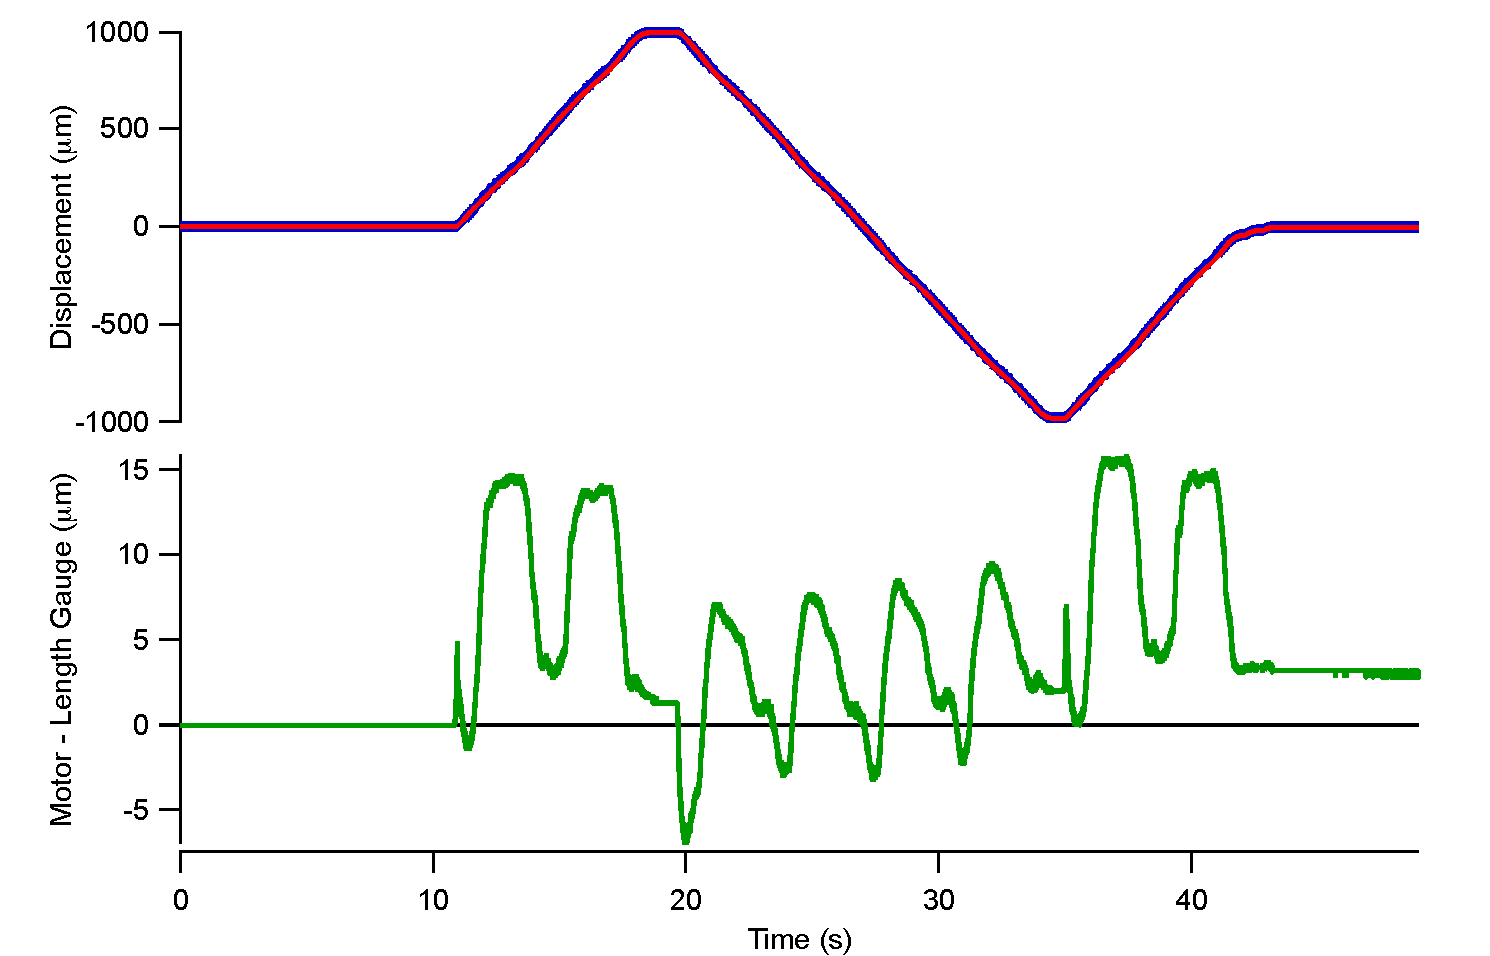
\includegraphics[width=1\textwidth]{Figures/motLGtrans.pdf}
\caption[Comparison of displacements measured by a motor encoder and a length gauge.]{\label{intRegionMotorLG}Displacement of the interaction region translation stage as measured by the motor encoder (blue) and a length gauge (red), and the difference in displacement measurements (green). Positive (negative) displacements correspond to retraction (extension) of the motor screw. Translating in the negative direction, corresponding to motor extension, is better for our experiments because the position error is lesser.}
\end{figure}



\begin{figure}
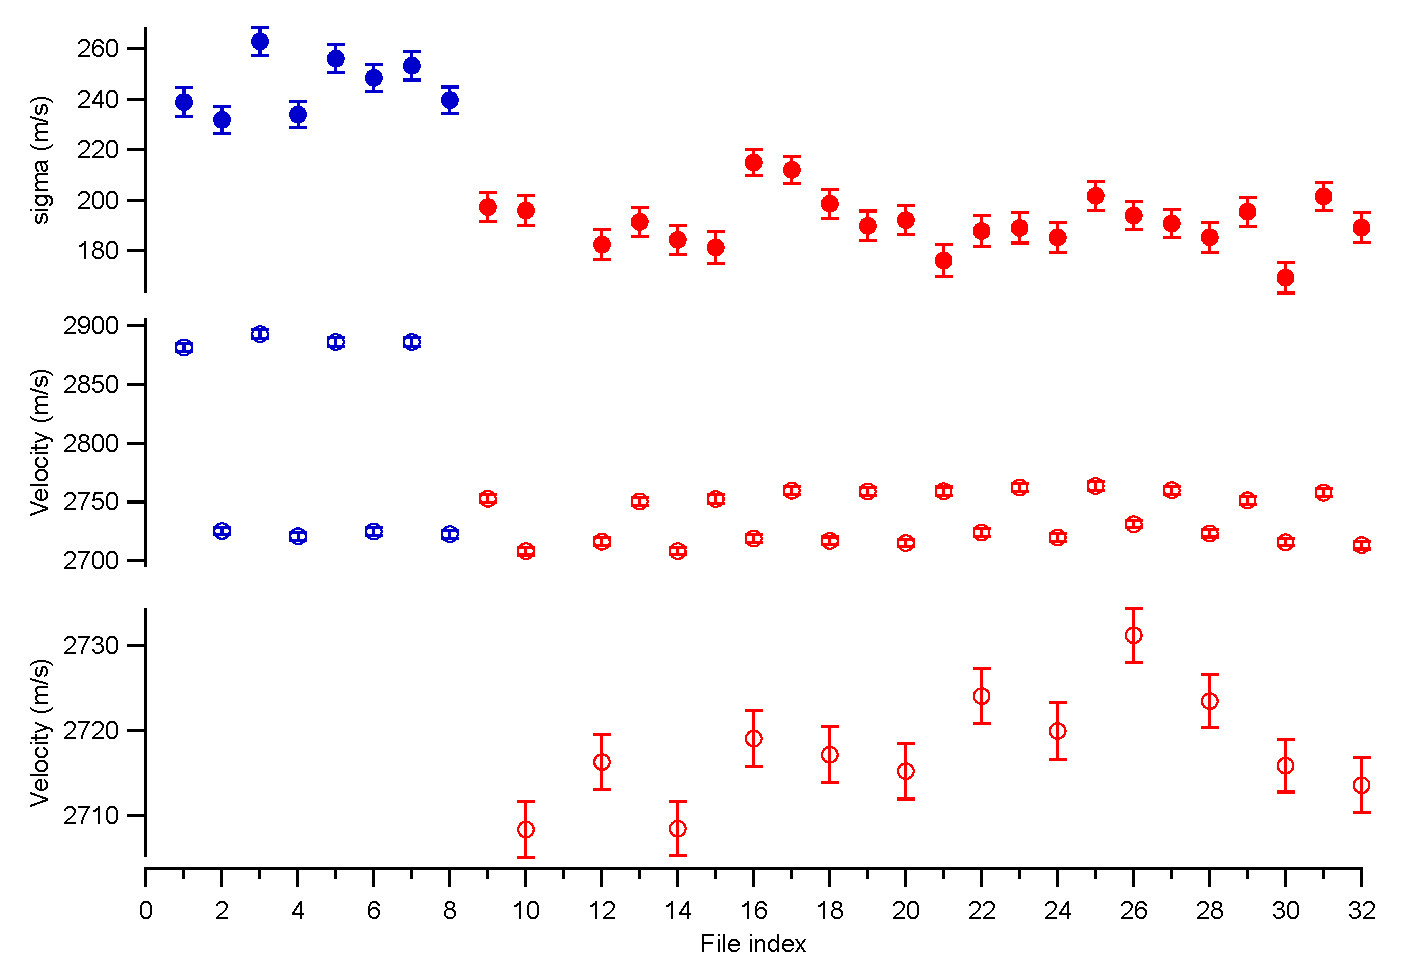
\includegraphics[width=1\textwidth]{Figures/velMotLG.pdf}
\caption[Atom beam velocities measured using a motor encoder and a length gauge.]{\label{velMotLG}Sodium atom beam velocity (open circles) and velocity distribution width (filled circles) using the detector motor (blue, files 1-8) or length gauge (red, files 9-32) to measure detector displacement. The up-down pattern in velocity reflects the fact that the motor direction was alternated and the translation stage exhibits stick/slip behavior. We only use the measurements corresponding to the extension of the motor screw (even numbered file indices), since this minimizes errors due to stick/slip of the translation stage. This subset of measurements yield $v=2717.8(6.5)$ m/s and $\sigma_v=190(11)$ m/s, where the uncertainties are the standard deviation and are statistical only.}
\end{figure}




%%%%%%%%%%%%%%%%%%%%%%%%%%%%%%%
\section{Reanalysis using a trimmed mean}
\label{trimMean2010}
I reanalyzed the 2010 polarizability data using a trimmed mean, so that the lowest and the highest 10\% of the data were discarded before calculating the mean and the standard error of the mean. This procedure is useful when outliers occur more frequently than a normal distribution of measurements would predict. Figure \ref{polPRAmeasurementsTrim}, Table \ref{polResultsTableTrim} and Table \ref{polRatiosTableTrim} show the results of this analysis. The statistical uncertainty of each polarizability measurement improves by about 20\%. As a result, the uncertainty of our measurements of $\alpha_\textrm{K}$ and $\alpha_\textrm{Rb}$ (determined by our ratio measurements of polarizabilities combined with the Ekstrom \etal measurement of $\alpha_\textrm{Na}$) improve slightly as well. These changes are well within the statistical uncertainty of the original measurements.


\begin{figure}
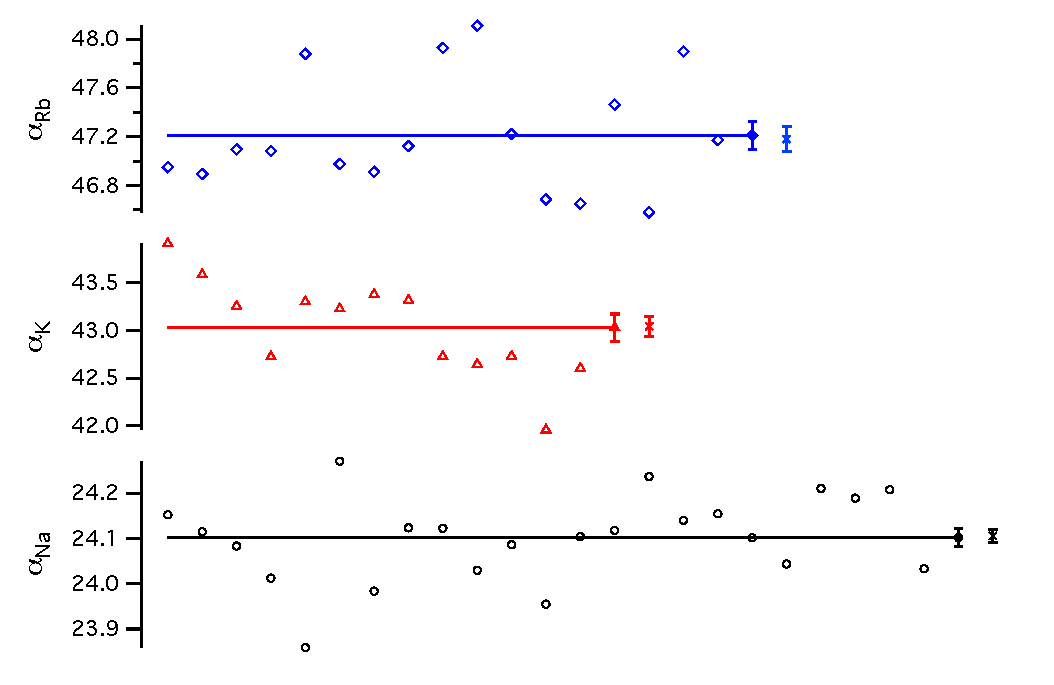
\includegraphics[width=1\textwidth]{Figures/polPRAdataTrim.pdf}
\caption[Multiple measurements of the polarizability of Na, K, and Rb and their trimmed means]{\label{polPRAmeasurementsTrim} Multiple measurements of the polarizability of sodium (circles), potassium (triangles), and rubidium (diamonds). The mean polarizabilities are denoted by filled markers and lines. The trimmed means are denoted by crosses. The error bars represent the standard error of the mean. Units are $10^{-24}$ cm$^3$. Final results are shown in Table \ref{polResultsTableTrim}.}
\end{figure}


\begin{table}
\caption[Measured absolute atomic polarizabilities using all data points and the central 80\%]{\label{polResultsTableTrim}Measured absolute atomic polarizabilities using all data points and the central 80\%. Also shown are the polarizabilities of K and Rb obtained using our ratios of polarizabilities using the central 80\% of the data (see Table \ref{polRatiosTableTrim}) combined with the sodium polarizability measurement from Ekstrom \etal \cite{Eks95}.}
\begin{center}
\begin{tabular}{c c | c | c}
\hline\hline
	& $\alpha_\textrm{abs All}$(stat.)(sys.) & $\alpha_\textrm{abs Trim}$(stat.)(sys.)  & $\alpha_{\textrm{Trim ratio \& Eks}}$(tot.)\\
\hline
Na & 24.11(2)(18) & 24.12(1)(18) & \\
K & 43.06(14)(33) & 43.08(11)(33) & 43.06(19)\\
Rb & 47.24(12)(42) & 47.21(10)(42)  &47.20(20)\\
\hline
\end{tabular}
\end{center}
\end{table}


\begin{table}
\caption{\label{polRatiosTableTrim}Measured atomic polarizability ratios with statistical uncertainties for the entire data set and the trimmed data set.}
\begin{center}
\begin{tabular}{c c c}
\hline\hline
 &  $\alpha_\textrm{ratio}$(stat.~unc.) \\
Atoms & All data & Trimmed \\
\hline
Rb/Na & 1.959(5) &1.958(4)  \\
K/Na    & 1.786(6) &1.786(5)  \\
Rb/K    & 1.097(5) &1.096(4)  \\
\hline\hline
\end{tabular}
\end{center}
\end{table}





%%%%%%%%%%%%%%%%%%%%%%%%%%%%%%%%%%%%
\section{Data acquisition system upgrades}
\label{newDAQ}

The 2010 polarizability measurements were accomplished by manually moving the interaction region and switching the high-voltage electrode on and off about once per minute. This quickly became mind-numbing, tedious work. Higher precision measurements of polarizability clearly demanded a more automated data acquisition system.

\begin{sidewaysfigure}
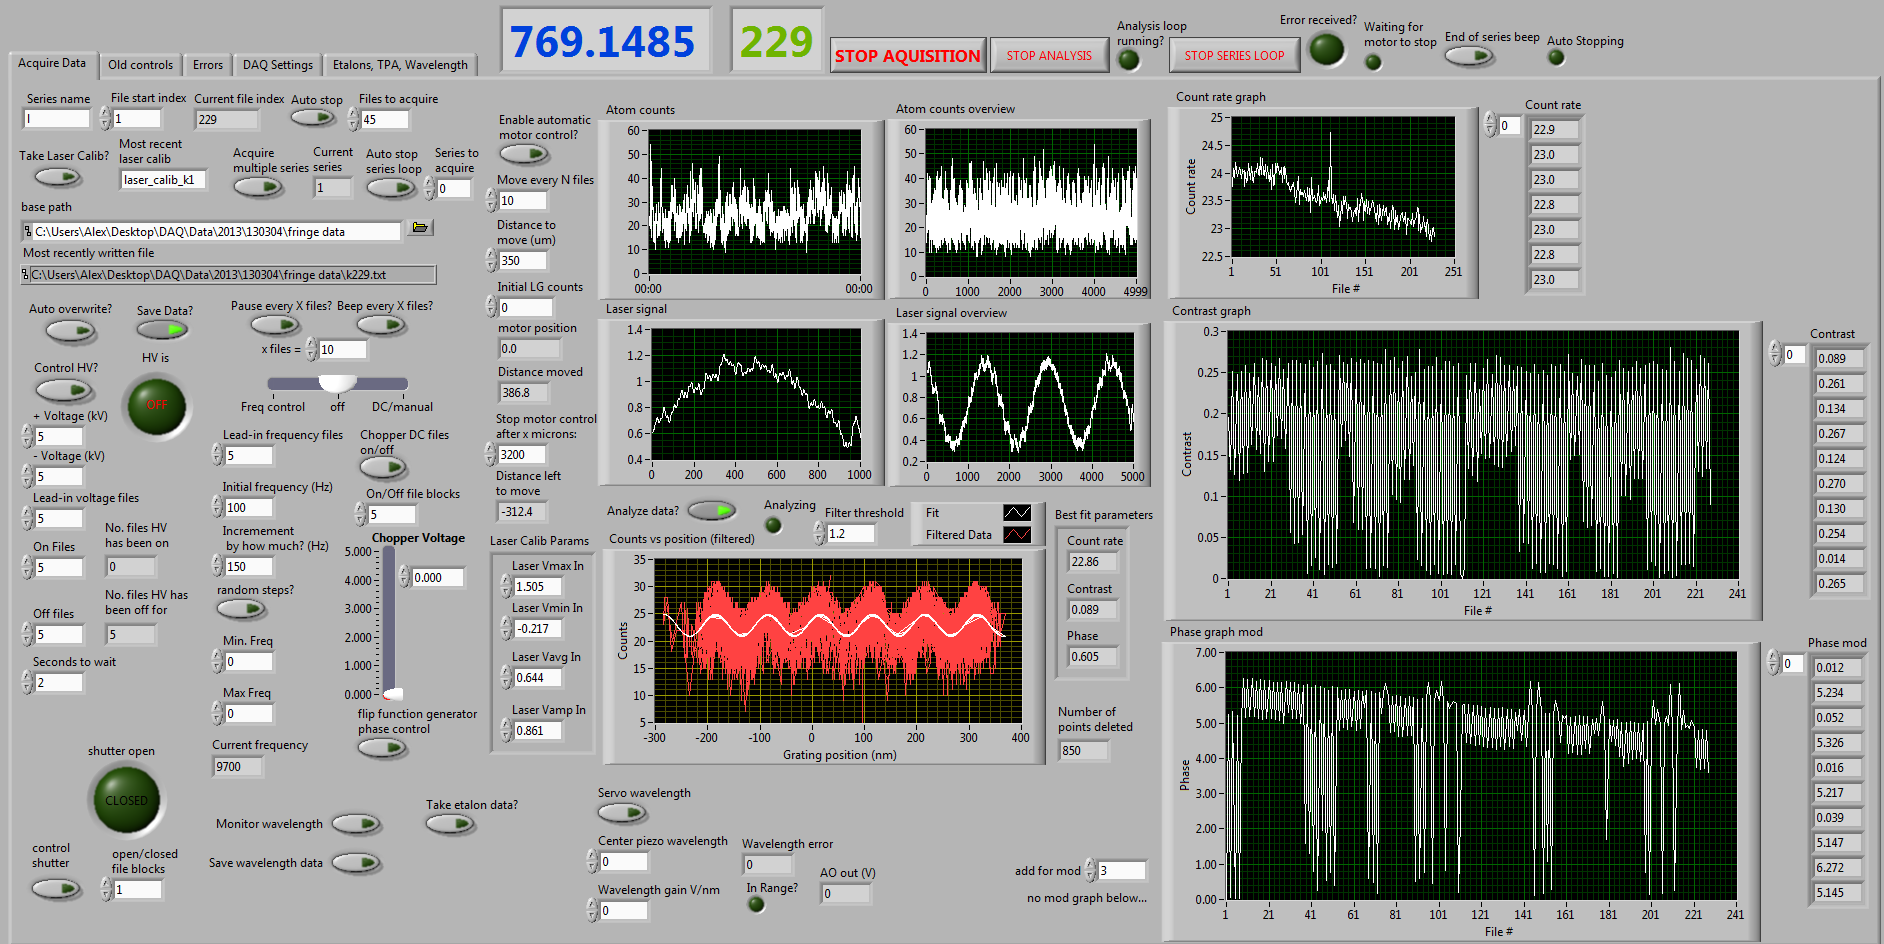
\includegraphics[width=1\textwidth]{Figures/daqScreenShotEdit.png}
\caption[Screenshot of the improved data acquisition system]{\label{DAQpicture}Screenshot of the data acquisition system. The left side contains experiment controls, such as data series name, the type of measurement (polarizability, velocity, or magic-zero wavelength), and high voltage settings. The middle section shows the atom count rate and laser interferometer data as a function of time and a plot of the interference fringe determined from the previous 5 s worth of data. Finally, the right side shows a history of the average count rate, contrast, and interferometer phase for the current data series. Additional tabs contain channel controls, error reporting displays, and some additional laser system monitors. While perhaps overwhelming at a glance, this suite of controls and instruments provides a significantly more powerful grasp of the experiment than the previous data acquisition system.}
\end{sidewaysfigure}


We developed a new data acquisition system in LabView 2010 with the ability to move and accurately record the distance traveled by any motor (via on-board quadrature decoding) in the atom beam machine and automatically control multiple high-voltage power supplies and a function generator. Figure \ref{DAQpicture} shows a screen shot of the data acquisition system. The new data-acquisition system uses a producer-consumer architecture to simultaneously record and analyze atom fringe data. This \emph{in situ} processing of atom fringe data has proven to be immensely valuable. Hardware controlled timing signals ensure that measurements of the atom beam count rate and the grating position are commensurate. A second screen enables viewing of the interferometer data from the optical table in our lab. 







%%%%%%%%%%%%%%%%%%%%%%%%%%%%%%%%%%%%
\section{Next-generation polarizability measurements}
\label{polChapterGradElg}

After publishing our 2010 polarizability measurements we designed a new experiment to improve both the precision and accuracy of polarizability measurements in our lab. We chose to replace the ground plane from the previous interaction region with a 2nd pillar. Figure \ref{IFMpillarsTrans} shows a schematic of the atom interferometer and a two-pillar interaction region. Figures \ref{newIntRegion2g} and \ref{intRegionNewPer} show a photo and a schematic of the new interaction region, respectively. The pillars are made of two 0.5 inch diameter rods separated by 3.81 mm. Figure \ref{twoPillarPolMeas} shows a measurement of cesium polarizability using the new interaction region.


As discussed in section \ref{polBrief}, the electric fields of the two regions are nominally identical, however, there are several advantages to the two-pillar geometry. First, two pillars allows us to measure phase shifts on both sides of the plane of symmetry in the electric field calculation. This in turn enables us to use phase shift data to independently determine both the polarizability and the position of the pillars relative to the atom beam. Measuring phase shifts on both sides of the symmetry plane also allows us to better control for the Sagnac phase shift. This is because the Sagnac phase shift makes the total phase shift closer to zero on one side of the pillars and farther from zero on the other, leading to an unambiguous signature. See Appendix A for a description of how the Sagnac phase shift effects the atom interferometer contrast and phase.


We also added a Heidenhain MT-2571 length gauge to measure the interaction region position. Irreproducibility in the interaction region position may have been a large source of the statistical error of the polarizability measurements in the first generation experiment. Section \ref{polLG} discussed the advantages of using a length gauge to measure displacement instead of relying on built-in rotary motor encoders.


Figure \ref{csPolNew} shows a single day of cesium polarizability measurements using the new electrodes, phase choppers for measuring atom beam velocity, and the new data acquisition system. Note the approximately 6 times improvement in statistical precision compared to our 2010 work, shown in Figure \ref{polPRAmeasurementsTrim}. Figure \ref{csPolVelDiff} shows consistent cesium polarizability measurements at three different atom beam velocities.



\begin{figure}
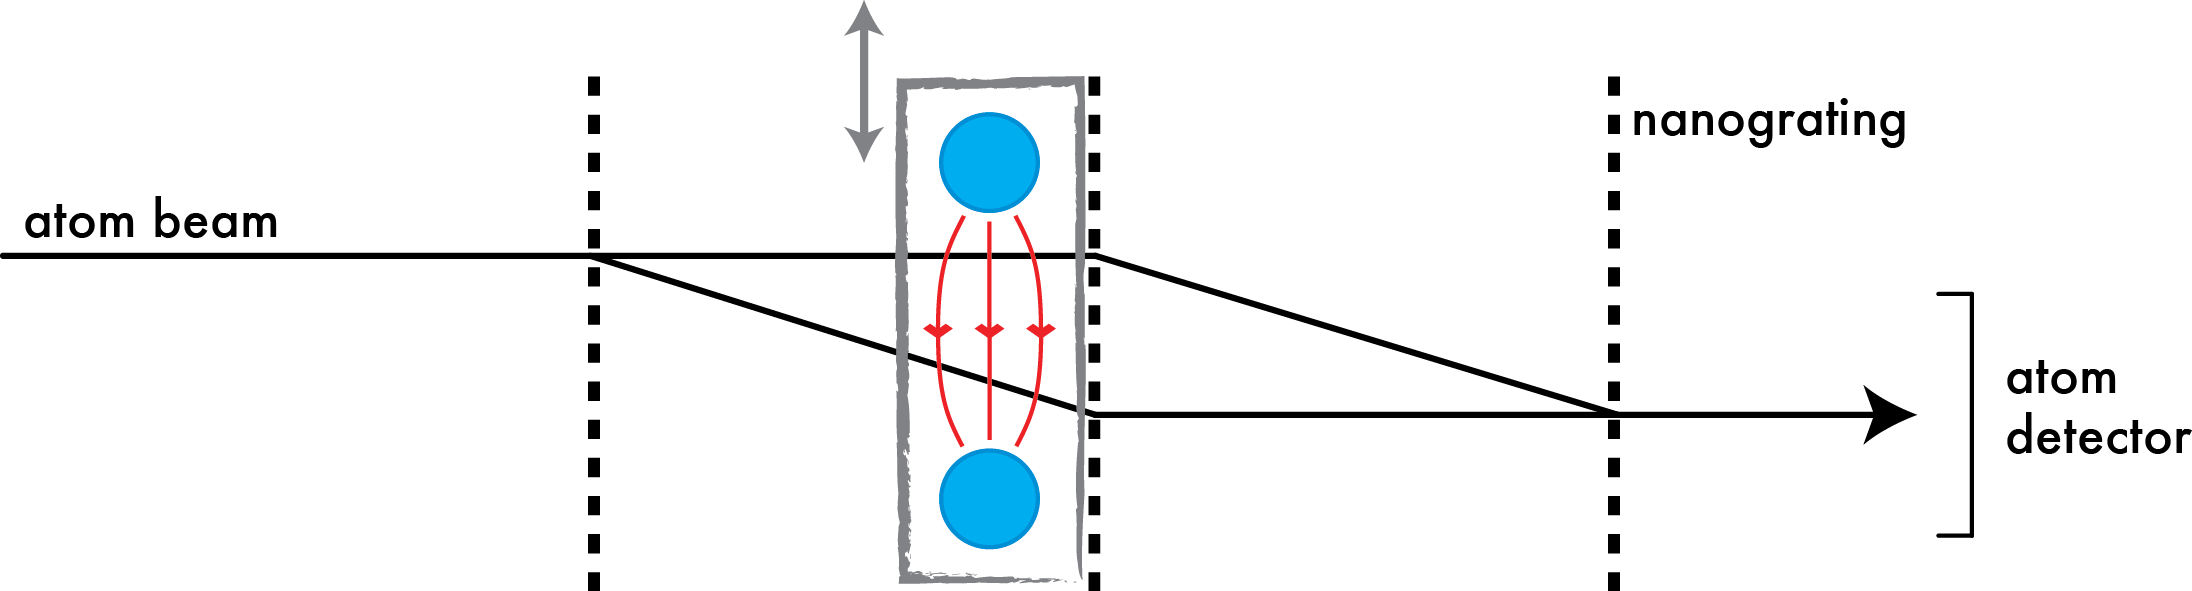
\includegraphics[width=1\textwidth]{Figures/IFMpillarsTrans.png}
\caption[Atom interferometer with two-pillar interaction region]{\label{IFMpillarsTrans}Atom interferometer with two-pillar interaction region. Measuring differential phase shifts as function of interaction region position, such as those shown in Figure \ref{twoPillarPolMeas}, allows us to determine the polarizability of an atom.}
\end{figure}


\begin{figure}
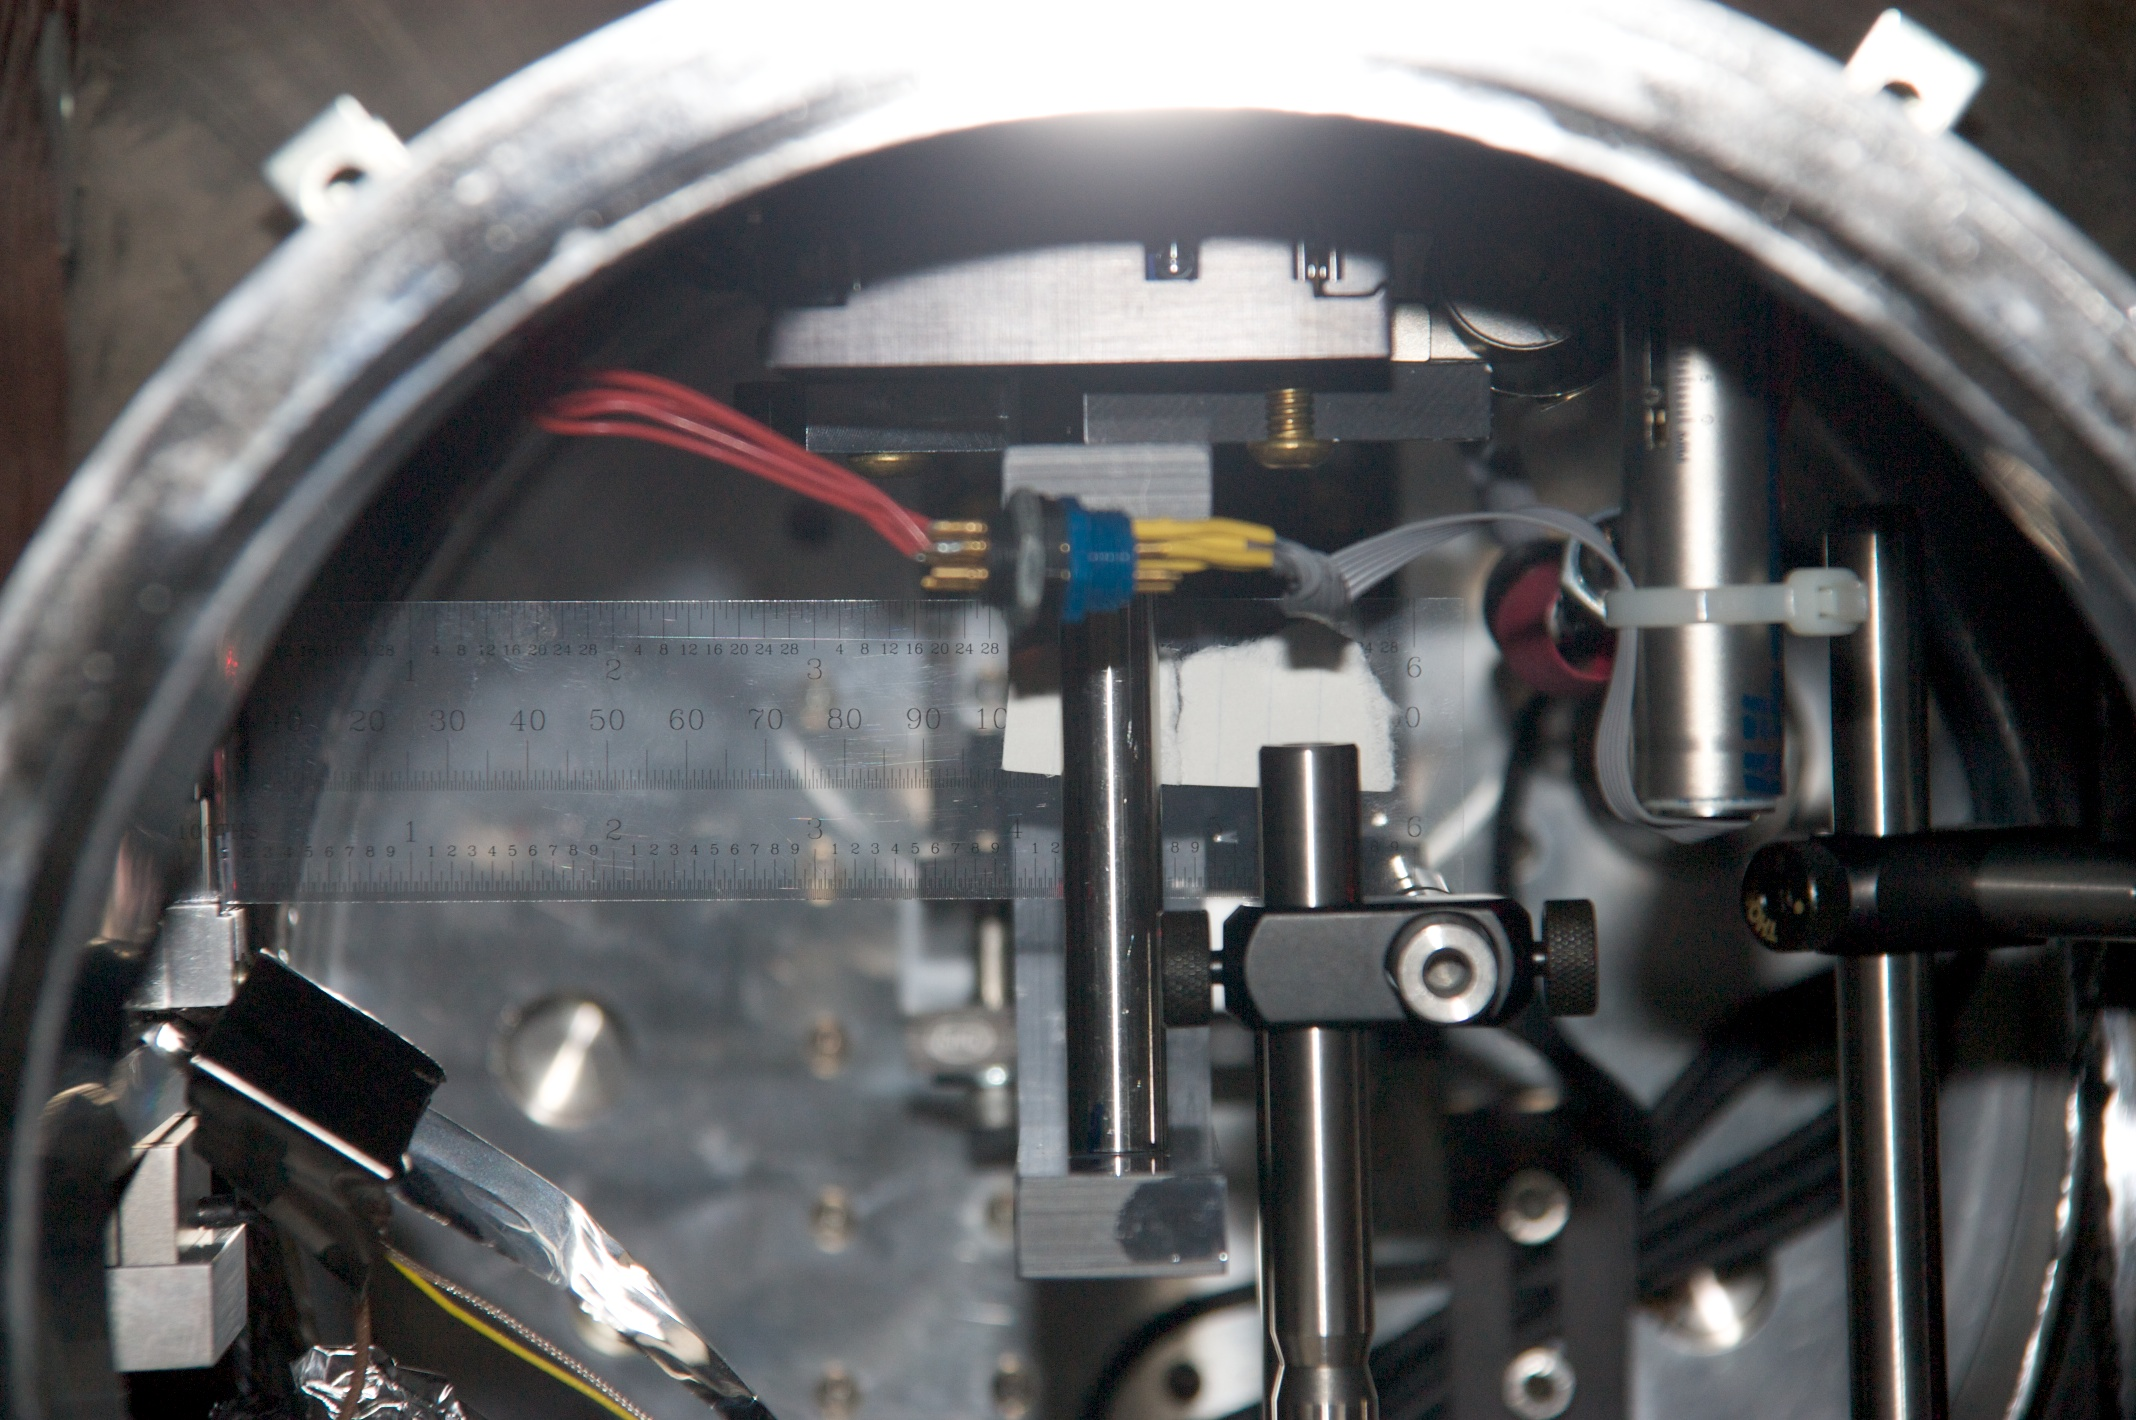
\includegraphics[width=1\textwidth]{Figures/intRegionNew2gMeas.jpg}
\caption[Measurement of the distance between the two-pillar interaction region and the 2nd nanograting]{\label{newIntRegion2g}Measurement of the distance between the two-pillar interaction region and the 2nd nanograting (left side, nearly edge-on).}
\end{figure}


\begin{figure}
\centerline{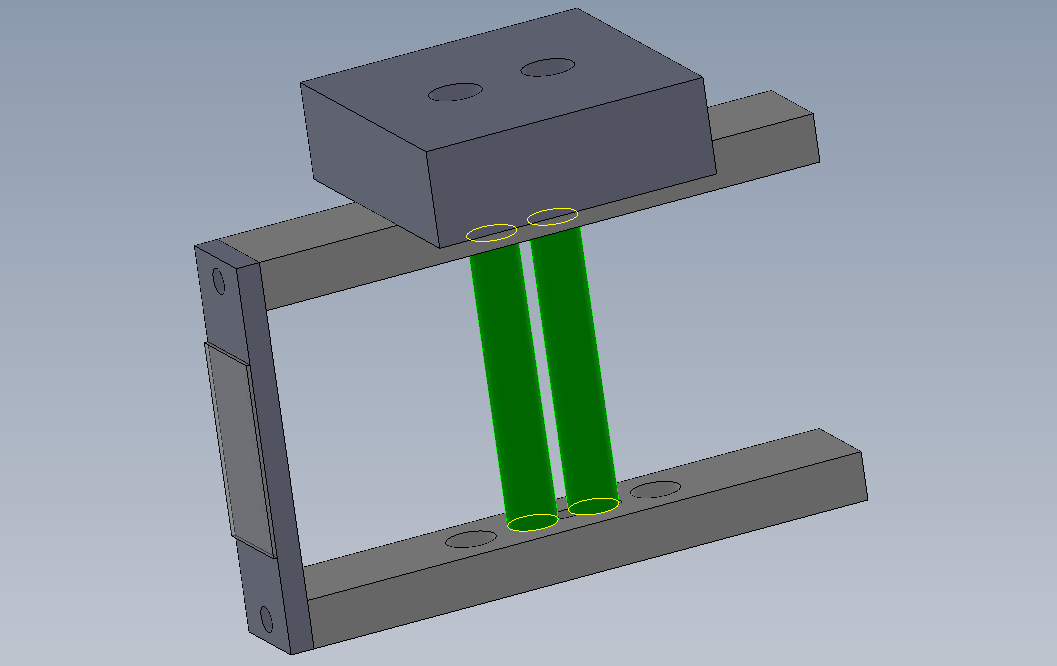
\includegraphics[width=0.75\textwidth]{Figures/intRegionNeweDrawings.png}}
\caption[Perspective rendering of the new interaction region]{\label{intRegionNewPer}Perspective rendering of the new interaction region. The electrodes (green) are held by PVC mounting bracket (light grey) and attached from below to a translation stage (dark grey). A microscope slide (semi-transparent) contacts a length gauge (not shown) for precise displacement measurements.}
\end{figure}


\begin{figure}
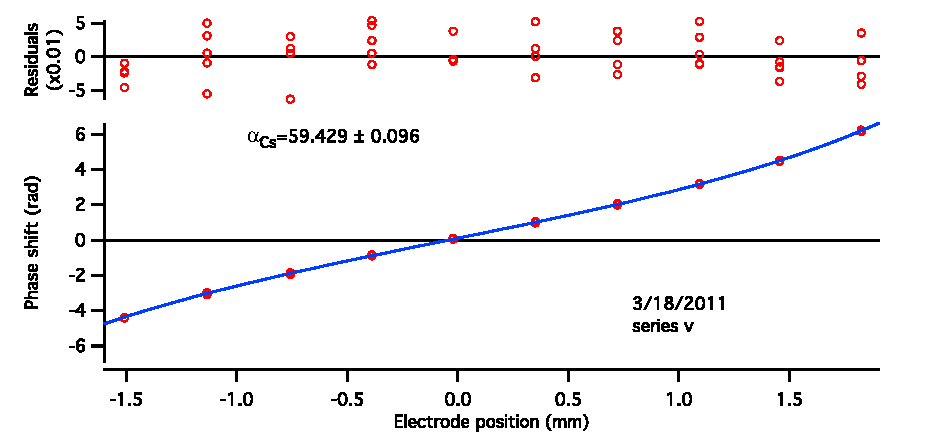
\includegraphics[width=1\textwidth]{Figures/twoPillarAlphaMeas.pdf}
\caption[Measurement of Cs polarizability using a two-pillar interaction region]{\label{twoPillarPolMeas}Measurement of cesium polarizability using a two-pillar interaction region. A least-squares fit to the phase shift data determines both the atomic polarizability and the atom beam position simultaneously. The reported uncertainty is statistical only.}
\end{figure}


\begin{figure}
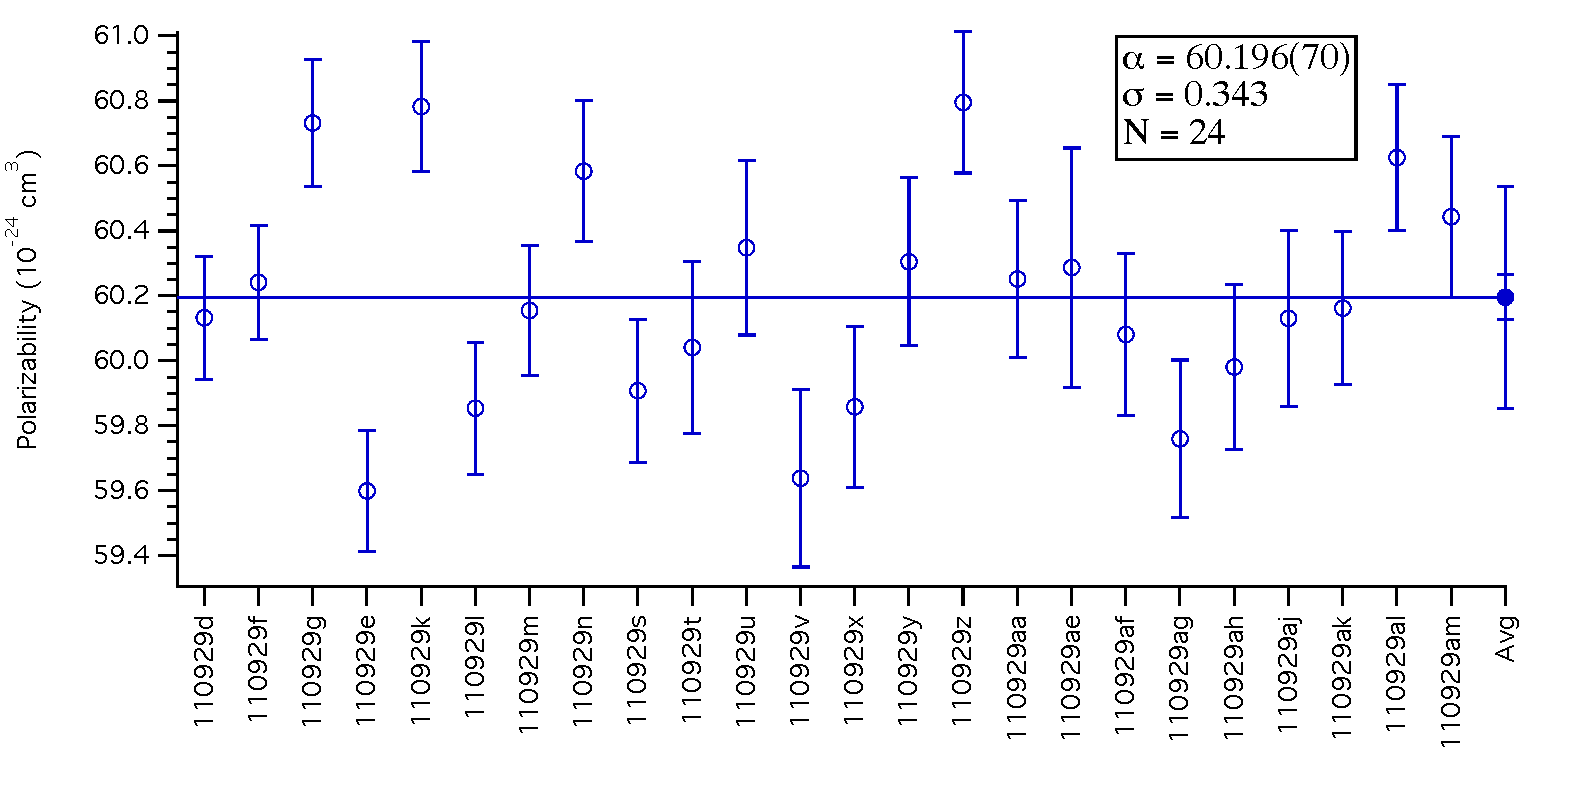
\includegraphics[width=1\textwidth]{Figures/csPol110929.pdf}
\caption[One day of polarizability measurements of Cs.]{\label{csPolNew}One day of polarizability measurements of cesium. The statistical precision (standard error of the mean) is 0.12\% (standard deviation of 0.5\%). However, the accuracy of this measurement is 1\% due to several uncalibrated parameters, such as the distance between the electrodes. The statistical uncertainty of each measurement is not used in determining the polarizability or the uncertainty, but is shown as a measure of consistency.}
\end{figure}


\begin{figure}
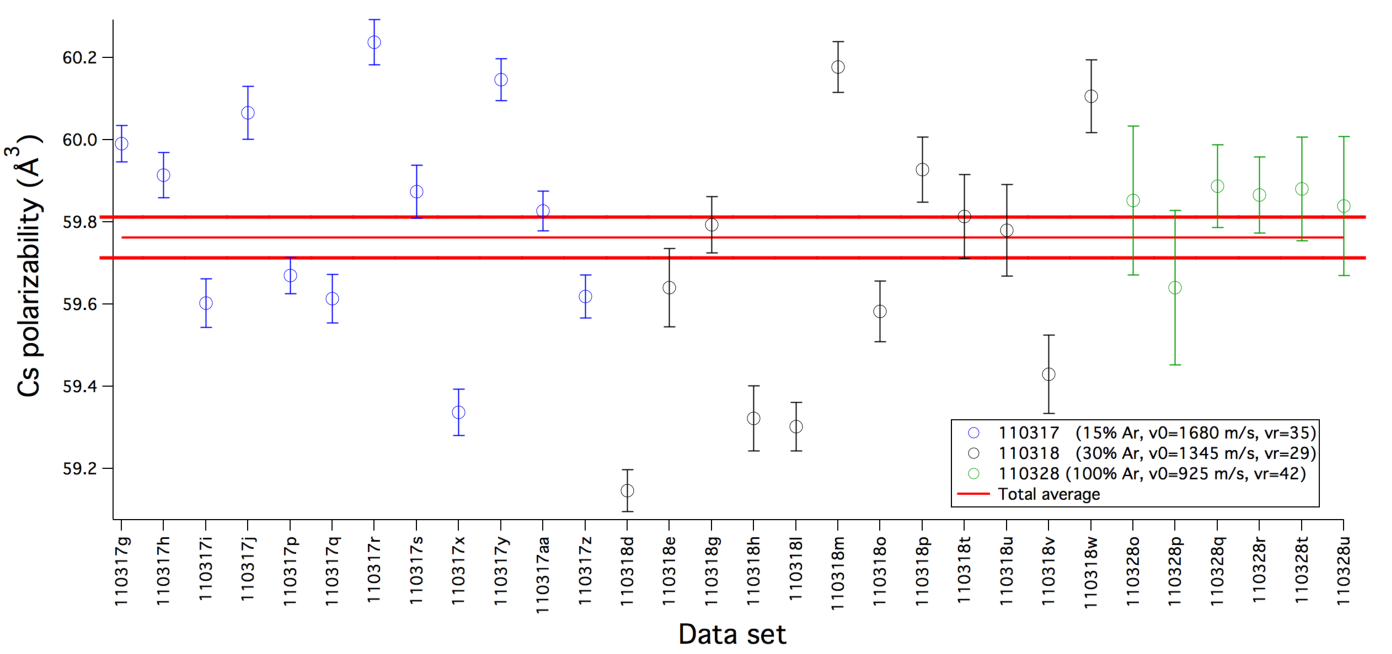
\includegraphics[width=1\textwidth]{Figures/csPolDifferentVels.pdf}
\caption[Consistent Cs polarizability measurements of at different velocities]{\label{csPolVelDiff}Consistent cesium polarizability measurements at three different velocities: 1680 m/s (blue), 1345 m/s (black), and 925 m/s (green). The total average and standard error of the mean is shown in red.}
\end{figure}


